\chapter{Goertzelův algoritmus}
\label{kap:goertzeluvalgoritmus}

\section{Diskrétní Fourierova řada}

Máme řadu $N$ hodnot libovolné posloupnosti. Fourier ukázal, že je možno převést
ji na $N$ hodnot nějaké frekvenční charakteristiky. \emph{Diskrétní Fourierova řada} přiřazuje časové periodické posloupnosti periody $N$,
posloupnost spektra, rovněž periodickou a rovněž periody $N$. Následující vzorec pochází z knihy \emph{Systémy a signály} od prof. Smékala\cite{smekal}.

\begin{myequation}
S_p[k] = \sum_{n=0}^{N-1} s_p[n] \eul^{-\jmag  k\frac{2\pi}{N}n},
\end{myequation}
\noindent kde \emph{k} $k.$ hodnota amplitudy ve spektru, nabývá hodnot $0..N-1, N$ je délka sekvence časové posloupnosti i délka spektra \emph{DFŘ}.
Řada má tedy určitý, omezený počet členů.

\section{Diskrétní Fourierova transformace - DFT}


Na rozdíl od \emph{DFŘ}, není obraz \emph{DFT} periodický. \emph{DFT} přiřazuje
časové posloupnosti délky $N$, posloupnost spektra, také délky $N$. S pomocí
\emph{DFŘ} by se vytvořil asi takto:
\begin{itemize}
\item Zperiodizování průběhu $s$, kde $s[n+lN] = s_p[n]$
\item Výpočet DFŘ.
\item Oříznutí spektra na jednorázovou posloupnost. 
\end{itemize}

\emph{DFT} zapisujeme jako

\begin{myequation}
\label{vztah:DFT}
S[k] = \sum_{n=0}^{N-1} s[n] \eul^{-\jmag  k\frac{2\pi}{N}n}.
\end{myequation}

I tento vzorec pochází z knihy prof. Smékala (\cite{smekal}).

\section{Goertzelův algoritmus}

Často je třeba řešit požadavek na zjištění složky spektra u určitém úzkém pásmu kmitočtů. Šlo by samozřejmě spočítat Fourierovou transformací celé spektrum a~vybrat jen ten kmitočet, který je pro nás zajímavý.
Další možností je spočítání jedné hodnoty z definice Fourierovy transformace, tak jako ve vzorci pro DFT (\ref{vztah:DFT}).
Myšlenkou \emph{Goertzelova algoritmu} je k tomuto účelu použít číslicové filtrace.
Goertzel použil druhou kanonickou strukturu (\ref{vztah:2kanonickastruktura}), realizovanou filtrem IIR (na obrázku \ref{obr:2kanonicka}).

\begin{myequation}
\begin{multlined}
\label{vztah:2kanonickastruktura}
v_1[n+1] = v_2[n] \\
v_2[n+1] = \frac{1}{b_2}(x[n]-b_1v_2[n]-b_0v_1[n]) \\
y[n] = a_2v_2[n+1] + a_1v_2[n] +a_0v_1[n] 
\end{multlined}
\end{myequation}

\begin{figure}
  \begin{center}
    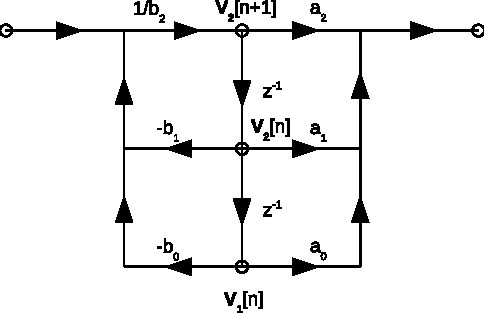
\includegraphics[scale=1]{obr/2kanonickastruktura}
  \end{center}
  \caption{Graf signálových toků druhé kanonické struktury.}
  \label{obr:2kanonicka}
\end{figure}


\section{Odvození Goertzelova algoritmu}

Následující odvození pochází rovněž z knihy prof. Smékala Systémy a signály \cite{smekal}.
\\
 Označme:

\begin{myequation}
\label{vztah:wn}
W_N = \eul^{-\jmag  \frac{2\pi}{N}},
\end{myequation}

pak

\begin{myequation}
\label{vztah:wnrovnost}
(W_N)^{-kN} = (\eul^{-\jmag  \frac{2\pi}{N}})^{-kN} = 1,
\end{myequation}

Protože člen (\ref{vztah:wnrovnost}) je jedna, můžeme s ním vynásobit definiční vztah Fourierovy transformace (\ref{vztah:DFT}), aniž by došlo ke změně.

\begin{myequation}
\begin{multlined}
\label{vztah:geotrzelsk}
S[k] = \sum_{m=0}^{N-1} s[m] W_N^{-kN} = (W_N)^{-kN} \sum_{m=0}^{N-1} s[m] W_N^{-kN} =\\
=\sum_{m=0}^{N-1} s[m] W_N^{-k(N-m)} = \sum_{m=0}^{N-1} s[m] \eul^{-\jmag\frac{2\pi}{N}k(N-m)}
\end{multlined}
\end{myequation}

Konečný tvar vztahu (\ref{vztah:geotrzelsk}) zjevně vypadá jako konvoluce
vstupní posloupnosti $x[n] = s[n]$ s impulsní charakteristikou číslicového filtru typu IIR


\begin{myequation}
\label{vztah:gertzelimpchar}
h[n] =  \eul^{-\jmag  k\frac{2\pi}{N}} = W_N^{-kN} = 1, n = 0,1,2..\infty
\end{myequation}

Impulsní charakteristika má komplexní koeficienty, což je zřejmé i z toho, že
spektrum DFT je také komplexní. Výstupní odezva potom je

\begin{myequation}
\begin{multlined}
\label{vztah:geotrzelyn}
y[n] = x[n]*h[n] = \sum_{m=0}^{\infty} s[m] h[n-m] = \sum_{m=0}^{\infty} s[m] W_N^{-k(n-m)} = \\
\sum_{m=0}^{\infty} s[m] \eul^{-\jmag k\frac{2\pi}{N}(n-m)}
\end{multlined}
\end{myequation}

Tento vzorec (\ref{vztah:geotrzelyn}) je ovšem nekonečná řada. Naštěstí není nutné
počítat do nekonečna, jelikož v hledané spektrální složce je jediný vzorek v čase $N$ roven

\begin{myequation}
\begin{multlined}
\label{vztah:geotrzelopak}
y[N] = \sum_{m=0}^{\infty} s[n] \eul^{-\jmag k\frac{2\pi}{N}(N-m)} =
\sum_{m=0}^{\infty} s[n] \eul^{-\jmag k\frac{2\pi}{N}N} \eul^{-\jmag k\frac{2\pi}{N}m} =
\sum_{m=0}^{N-1} s[n] \eul^{-\jmag k\frac{2\pi}{N}m} =\\
 S[k]
\end{multlined}
\end{myequation}

Přenosová charakteristika filtru typu IIR s impulsní charakteristikou (\ref{vztah:gertzelimpchar}) je prvního řádu

\begin{myequation}
\begin{multlined}
\label{vztah:geotrzelhz}
H(z) = \sum_{n=0}^{\infty} h[n]z^{-n} =  \sum_{n=0}^{\infty} \eul^{-\jmag k\frac{2\pi}{N}n} z^{-n}= \sum_{n=0}^{\infty} ( \eul^{-\jmag k\frac{2\pi}{N}} z^{-1} )^{n} =\\
 \frac{1}{1-\eul^{-\jmag k\frac{2\pi}{N}}z^{-1}} = \frac{z}{z-W_N^{-k}}
\end{multlined}
\end{myequation}

Nevýhodou zcela jistě je skutečnost, že se v přenosové funkci vyskytují komplexní
koeficienty. Následující úprava vztahu (\ref{vztah:geotrzelhz}) tohle řeší. Daň za
možnost práce s jen reálnými čísly je přenosová funkce druhého řádu.

\begin{myequation}
\begin{multlined}
\label{vztah:geotrzelodvoz}
H(z) = \frac{1}{1-W_N^{-k}z^{-1}} = \frac{1}{1-W_N^{-k}z^{-1}} . \frac{1-W_N^{k}z^{-1}}{1-W_N^{k}z^{-1}} =\\
 \frac{1}{1-\eul^{-\jmag k\frac{2\pi}{N}z^{-1}}}
. \frac{1-\eul^{-\jmag  k\frac{2\pi}{N}z^{-1}}}{1-\eul^{-\jmag  k\frac{2\pi}{N}z^{-1}}} =
\frac{1-\eul^{-\jmag  k\frac{2\pi}{N}z^{-1}}}{1 - (\eul^{-\jmag  k\frac{2\pi}{N}+\eul^{-\jmag k\frac{2\pi}{N}})z^{-1} +z^{-2}}} = \\
\frac{1-\eul^{-\jmag  k\frac{2\pi}{N}z^{-1}}}{1-2\cos{k\frac{2\pi}{N}}z^{-1}+z^{-2}} =
\frac{z^{2}-\eul^{-\jmag  k\frac{2\pi}{N}z}}{z^{2}-2\cos{k\frac{2\pi}{N}}z+1} = 
\frac{a_2z^{2}+a_1z+a_0}{b_2z^{2}+b_1z+b_0}
\end{multlined}
\end{myequation}

Výsledek porovnáme se stavovými rovnicemi (\ref{vztah:2kanonickastruktura}) A zjistíme tak následující koeficienty.

\begin{myequation}
\begin{aligned}
\label{vztah:geotrzelkoef}
b_2 &= 1,&&\\
b_1 &= -2\cos{k\frac{2\pi}{N}},&&\\
b_0 &= 1,&&\\
a_2 &= 1,&&\\
a_1 &= -\eul^{-\jmag  k\frac{2\pi}{N}},&&\\
a_0 &= 0
\end{aligned}
\end{myequation}


Jejich dosazením  do (\ref{vztah:2kanonickastruktura}) dostaneme...

\begin{myequation}
\begin{aligned}
\label{vztah:geortzelstavrovnice}
v_1[n+1] &= v_2[n], &&\\
v_2[n+1] &= x[n]+2\cos{k\frac{2\pi}{N}}v_2[n]-v_1[n], &&\\
y[n] &= v_2[n+1] -(\cos{k\frac{2\pi}{N}} -\jmag  \sin{k\frac{2\pi}{N}}) v_2[n], &&\\
\end{aligned}
\end{myequation}


\begin{figure}
  \begin{center}
    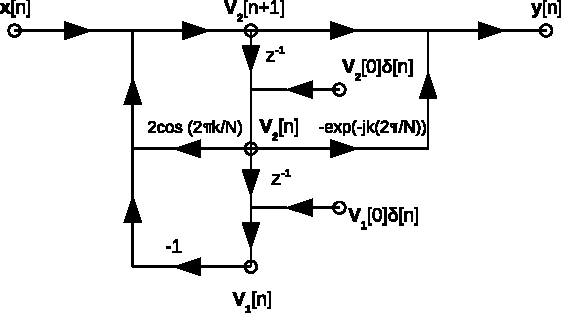
\includegraphics[scale=1]{obr/goertzel}
  \end{center}
  \caption{Graf signálových toků Goertzelova algoritmu ve 2. kanonické struktuře.}
  \label{obr:goertzelova2kanonicka}
\end{figure}

Výhodou této struktury je, že nám stačí ve smyčce počítat jen proměnné
$v_1$ a $v_2$. Výstup $y$ se počítá jen jednou, při posledním průchodu cyklem, kdy $n=N$. Počáteční hodnoty $v_1$ a $v_2$ jsou nulové. Komplexní operace tak bude
provedena pouze jednou a to až na závěr.